\chapter{Scrambling}\label{ch:Scrambling}
Security is not only about cryptography. But there is a main reason why 
cryptography is attacked , and that is because there is a very low chance 
of being detected. There will be no traces of the attack, since the attacker’s 
access will look just like a legitimate /"good" access. 

This can be compared to a real-life break-in. The break-in will be noticed if 
the thief breaks in using a crowbar. If the thief, on the other hand, would be 
to pick the lock, there is a possibility that you will never notice that your 
security has been breached \citep{Schneier:2003}.

There are many rules concerning cryptography, as there are to all sciences. 
The one I found most noteworthy was that one is to always assume that someone 
is "out to get you". Because of this, \citet[pp. 12--14]{Schneier:2003} say that 
we always need  to look for possible ways to break systems, to make sure that
we are safe.

\section{What is the need for cryptography?}
If we communicate without encrypting the data we are sending, someone 
else will most likely be eavesdropping. For most people this isn’t a problem, 
but in some instances sending secure messages can be extremely important. One 
example is communication during war, where a single piece of intelligence might 
turn the tide of the entire war. Another example is sending manuscripts, and 
drafts of books over the internet. These are some of the reasons as to why we 
want to encode messages.

Another reason for scrambling is to reduce the number of adjacent data-bits with 
the same value, as in long strings of zeros or ones. 

%Balancing the amount of 
%zeros and ones gives a DC balance, which means that the signal is stronger when 
%sent.

\section{Scrambling or Encrypting}
The difference between scrambling and encryption is that scrambling is the
way we generate the secret control word (key) which is used when we make the
data unreadable to outsiders while encryption is the way we protect the control 
word during transmission.

\Warning[Todo]{Det här måste jag bli säkrare på}
% What is the difference between scrambling and encryption? 

\section{Data packets}\label{sec:Data}
The data processed by the DVB systems is sent in data packets. All of them are 
created from ES packets (elementary streams) which generally is the output from 
an audio or video encoder. The ES packets are then packeted into PS, TS or PES 
packets and then distributed. There are three different ways of packing data, 
but only two of them are commonly used. The types are called TS, PS and PES. PS 
packets are used while data isbeing stored, while TS and PES are used when data 
is being transmitted. The ones interresting when working with DVB are therefore 
the TS packets as well as the PES packets.

\subsection{TS packets}
TS packets are the ones used by the DVB society, possibly due to their fixed 
lenghts. TS packets have got a length of 188 bytes with a 4 byte long header, 
meaning the payload consists of 184 bytes. The layout of a TS packet can be 
viewed in figure \ref{img:Package}.

\begin{figure}
  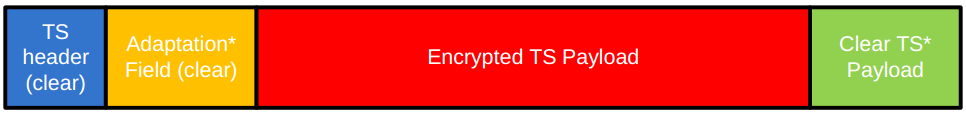
\includegraphics[width=\textwidth]{TSpacket}
  \caption{General layout of a data packet \citep{DVB:2013}}
  \label{img:Package}
\end{figure}

The building blocks that the TS packets consist of are:

\begin{itemize}
\item Header
\item Adaptation field - might not exist
\item Encrypted payload - might not exist
\item Clear payload
\end{itemize}

The header consist of information regarding the packet. The header provides 
information as to whether there is an adaptation field in the packet, what id 
the packet has, the sync byte and two bits telling us whether the data is 
scrambled using an odd or even key, if it is scrambled. The header is never to 
be encrypted and is always found in the beginning of the packets.

The adaptation field is a padding that you input when the end of the data is not 
aligned with the end of the TS packet. This is done to make sure that the TS 
packet is filled. We only find adaptation fields we are working with the last 
string of data, if the data does not align. Adaptation fields are not encrypted.

We are prone to end up with clear bytes of data in the TS packets when we work 
with block ciphers, since block ciphers only encrypt fixed sizes of data. The 
clear data is always located at the end of the packets and can in a worst case 
scenario be up to one byte smaller than the block size, since that will be the 
largest amount of bytes that does not fill an entire block. The encrypted 
payload is always located in front of the clear payload 
\cite[pp. 10--11]{DVB:2013}.

\subsection{PES packets}
The PES packets have varying lengths of up to 64 KBytes.

PES-packets can be of any size less than 64 Kbytes. They are often packed into 
TS packets when distributed, due to the strength of the TS packets. The payload
data in the TS packets consists of the entire PES packets, which consists of the 
header and the data. PES packets do not use adaptation fields, since they can be 
of more or less any length, as long as the packet do not exceed 64 KBytes.

\begin{figure}
  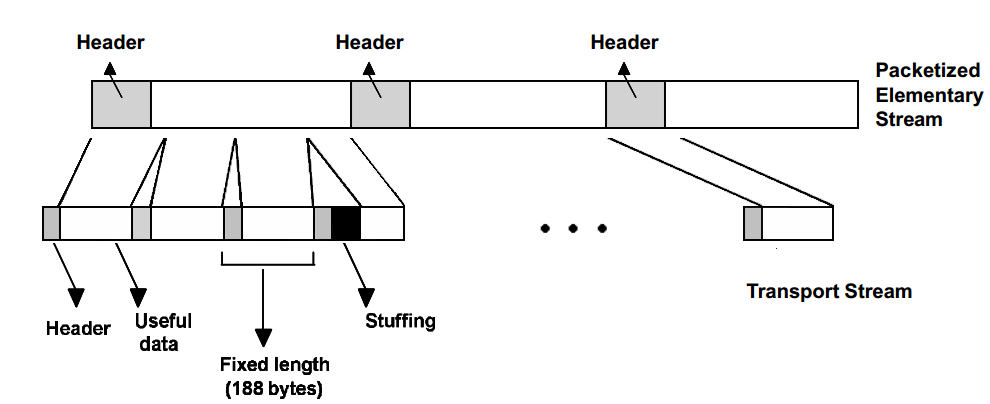
\includegraphics[width=\textwidth]{PES.png}
  \label{img:PES}
  \caption{PES packet derived from TS packets (inspiration for the image 
taken from \citep[p. 9]{ETR:289} ) }
\end{figure}

\section{Encryption and Decryption}
There are two things that you need when you encrypt and decrypt messages. Those 
are the algorithm as well as the key. There are plenty of ways to encrypt 
messages, but there are two ways of sharing the encryption-key. The first method 
being the symmetric-key encryption, and the second method being the public-key 
encryption.

\subsection{Symmetric-key encryption}
The symmetric-key encryption uses the same key to encode and decode messages. 
Distrubution of the key, when using the symmetric-key encryption is troublesome 
and the fact that both parties need access to the same secret key is a major 
drawback of the symmetric key encryption, as compared to the public-key 
encryption method. Sending the key in an email is a bad idea, since the persons 
who wants to read our messages  most likely already will be listening, and they 
will therefore obtain the key as well as the means to decode the messages we 
send.

\subsection{Public-key encryption}
The public-key encryption uses a public key that anyone can look up, and a 
secret key that only one person knows \citep[pp. 25--32]{Simmons:1992}.
For instance say that the two persons, Bob and Alice, want to communicate. 
Bob produces a keypair \(P_{Bob}\) (Bob’s public key) and \(S_{Bob}\) 
(Bob’s secret key) and publishes \(P_{Bob}\) for anyone to see. When Alice wants 
to send Bob a message, she looks up Bob’s public key \(P_{Bob}\), which she then 
uses to encode her message. When she sends Bob the message, Bob decodes the 
message using his secret key \(S_{Bob}\) \citep{Schneier:2003}.

\subsection{Combination}
The big question now is why we would use anything other than the public-key
encryption, since it seems secure and easy to manage. The reason is that the 
public-key encryption is not as effective as the symmetric-key encryption. 
It is common to use a combination of those two since an easy and effective way 
to encrypt messages is what we desire. To do this we use a symmetric-key 
algorithm to encode the plaintext into ciphertext, and then we use the 
public-key encryption to encode the symmteric-key we used when encoding the 
plaintext. This encoded key is then sent together with the ciphertext to the 
recipient, who uses the secret key to decode the symmetric key, which is then used to decipher ciphertext and obtain the plaintext.

Decryption is often performed by reversing the encryption. You need to know the 
algorithm, preferably through a mathematical representation, to calculate how 
to obtain the plaintext from the ciphertext. A description of how this is done 
for the CBC-mode (described in \ref{sec:BlockCipher}) is described in 
\ref{sec:CBCcalc} in appendix \ref{app:misc}. We assume that we know the 
decryption algorithm here for simplicity. \Warning[Source]{feels like a given, but still}

\section{Ciphers}
A cipher is the same as an algorithm, that operates on either plaintexts or 
ciphertexts to perform encryption or decryption. Figure \ref{img:ciphers} 
describes how they can be split into smaller groups.

\begin{figure}
  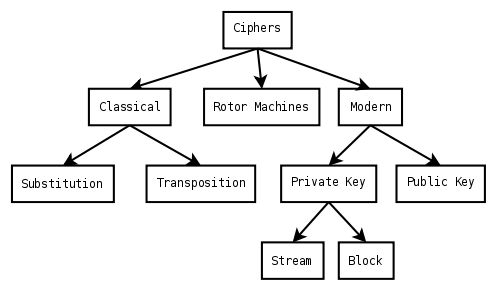
\includegraphics[width=\textwidth]{cipher.png}
  \caption{Different kinds of ciphers \citep{CipherTax:2013}}
  \label{img:ciphers}
\end{figure}

There are mainly two kinds of ciphers that are used when designing modern 
cryptosystems. Those ciphers are called block ciphers and stream ciphers. 
Many systems use a combination of block ciphers and stream ciphers to provide 
security. 
\Warning[Source]{At least the CSA uses it. But you need a source if you want 
this to be here}

\subsection{Block cipher}\label{sec:BlockCipher}
A block cipher operates on blocks where each block consists of a fixed number 
of bytes. This might cause a need for padding the blocks, in case the plaintext 
contains a number of bytes that is not even with the blocksize. Block cipher 
often use itself of a combination of S-boxes and P-boxes in a so-called 
SP-network (Figure \ref{img:SPNetwork}).

There are many modes of block ciphers, but the two recommended by 
\citet{Schneier:2003} are the CBC-mode and the CTR-mode.

CBC stands for \emph{cipher block chaining} and is performed by first encrypting 
the result of an XOR between an IV and the plaintext. This is the ciphertext 
that corresponds to the first plaintext. This is then put into an XOR with the 
next plaintext, and then encrypted \citep[pp. 109--111]{Stinson:2006}. For 
reference, see image \ref{img:CBCmode} in appendix \ref{app:misc}.

CTR stands for \emph{counter}, and refers to the way the IV is generated. The
counter outputs a value, which is encoded with the key. The output is then run 
in an XOR together with the plaintext, producing the ciphertext. The counter is 
then incremented and the procedure is iterated \citep[p. 111]{Stinson:2006}.

\subsection{Stream cipher} \label{sec:StreamCipher}
Stream ciphers work on a stream of data (as implied by the name). They usually 
consist of some kind of a keystream generator which performs a modulo 2 addition
with the data \cite[pp. 67]{Simmons:1992}. An effective implementation of the 
stream cipher is to use a linear feedback shift-register which uses the current 
internal state (key) to produce the next state by a simple XOR-addition between 
two or more of the bits in the state. This is mainly used because of how easy
it is to construct in hardware \citep{LFSR:2008}.

%\citet[{Simmons:1992} claims that there are four main approaches to constructing a stream-cipher; The information-theoretic approach, the system-theoretic approach, the complexity-theoretic approach and randomized stream ciphers.

\section{Confusion and Diffusion}\label{ch:ConfDiff}
Two properties that are needed to ensure that a cipher provides security are 
confusion and diffusion \citep{Shannon:1949}. Note that a cipher is not secure 
just because these two properties are obtained.

\emph{Confusion} refers to making the relationship between ciphertext and key as 
complex as possible. \emph{Diffusion} refers to replacing and shuffling the 
data, to make it impossible to analyze data statistically. This is usually done 
by performing substitutions and permutations in a simple pattern multiple times. 
This can easily be done by using an SP-network (S-box / P-box network) 
\citep[pp. 74--79]{Stinson:2006}. The very first, as well as last step, of 
SP-Networks is usually an XOR between the subkey and the data. This is called 
\emph{whitening}, and is according to \citet[p. 75]{Stinson:2006} regarded as a 
very effective way to prevent encryption/decryption without a known key. 
The goal of this is to make it hard to find the key, even though one has access 
to multiple plaintext/ciphertext pairs produced with the same key 
\citep{Shannon:1949}.

\subsection{S-boxes}
The S-box is one of the basic components that is used when creating ciphers. 
An S-box takes a number of input bits and creates a number of output bits in 
a non-linear fashion \citep[pp. 74--75]{Stinson:2006}. They can effectively be 
implemented as lookup tables. Each input has to correspond to a unique output, 
to make sure that the input can be recreated in the descrambler.

%One way of making it harder to find the relation between the input and the output is to place adjacent bits far from each other in the lookup table 
\Warning[TODO]{You need sources for this!}. 

% CONFUSION OR DIFFUSION?

\subsection{P-Boxes}
The second basic component used in cryptography is the P-box. A P-box 
shuffles/rearranges the order of given bits. This can be viewed in the 
SP-network in figure \ref{img:SPNetwork}, where the P-box is represented by the 
dotted rectangle in the middle.

\begin{figure}
  \begin{center}
    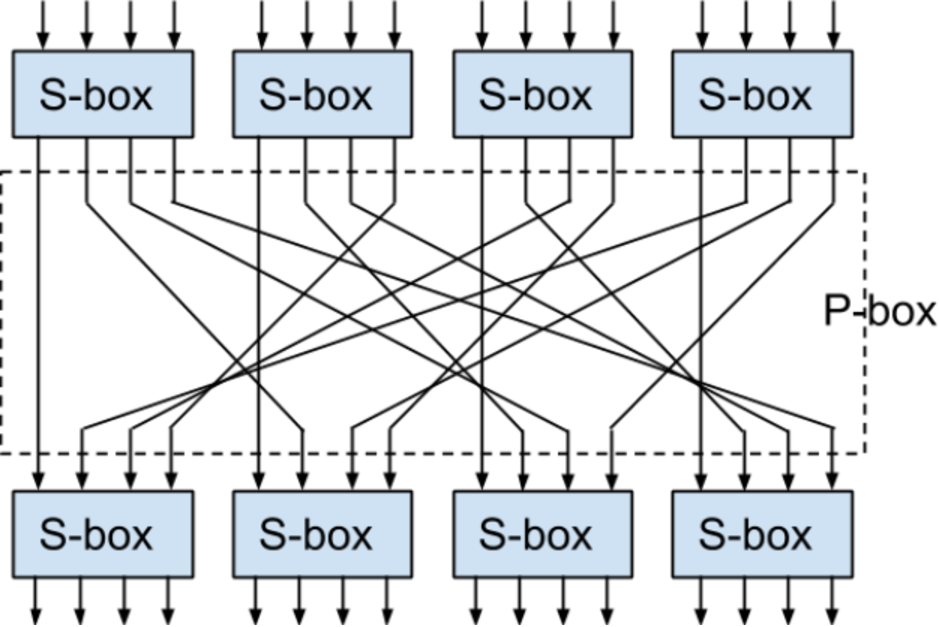
\includegraphics[width=0.8\textwidth]{SPnetwork}
    \caption{SP-Network}
    \label{img:SPNetwork}
  \end{center}
\end{figure}

%CONFUSION OR DIFFUSION?

\section{Secrecy}
Although encryption is important, as well as the strength of the encryption, 
keeping the algorithm secret is never a good idea. A simple mistake when 
designing an algorithm might turn an encryption that would have been strong,
incredibly weak. It is therefore a bad idea to use small scale algorithms  
(designed for the use of just a few persons for instance). If you instead 
use an open algorithm, faults will most likely be discovered and fixed by 
experienced cryptographers \citep[pp. 23]{Schneier:2003}. Keeping the key, 
which is used to encrypt the data, secret is what is important.
